%\chapter{Introduction}
\label{chap:intro}
\section{Motivation}

\change{Significant advancements in the fields of micro and nanotechnology in recent decades have enabled controlling heat flow in microscopic scale} \cite{cahill03,cahill14}. \change{Such thermal engineering has enabled, e.g. increasing the efficiency of thermoelectric heat-to-electricity converters} \cite{snyder08,vineis10,shakouri11}, \change{designing nanoporous aerogels for thermal insulation in buildings \cite{baetens11} and spacecraft \cite{jones06}, and alleviating the problem of overheating in microprocessors \cite{}.} Accurate temperature control is expected to enable also completely new technologies such as phase-change memory \cite{lankhorst05}, heat-assisted magnetic recording \cite{pan09}, tumor therapy based on nanoparticle heating \cite{avedisian09}, and information processing using thermal energy \cite{li12_rmp}. For all such applications, a solid understanding of energy transfer processes in nanoscale is necessary. %To tackle the power problem and to enable efficient thermal engineering, thorough understanding of heat transfer mechanisms are required. 
%  temperature-related 

% the engineering of nanomaterials with improved electrical, thermal and optical properties. This miniaturization has drawn considerable attention into thermal effects \cite{cahill03,cahill14}, which are crucial for, e.g., designing more efficient thermoelectrics \cite{snyder08,vineis10,shakouri11} and tackling the problem of overheating in microprocessors \cite{pop06_ieee,pop10}. 

% Nanoscale physics richer in nanoscale

Microscopically, energy is transferred in solid-state systems by lattice vibrations, electromagnetic fields, and electrons \cite{chen}. Compared to macroscale, where thermal transfer is characterized by constitutive material parameters such as thermal conductivity, heat transfer in nanoscale is enriched by the presence of intrinsic length scales competing with the system size \cite{chen}. For example, when the \change{the intrinsic scattering length or the wavelength of heat carriers exceeds the system size}, classical laws such as Fourier's law of thermal conduction \cite{fourier} and Planck's law of thermal radiation \cite{planck00a} break down, giving rise to novel phenomena such as thermal conductance quantization \cite{rego98,angelescu98,schwab00} and near-field enhancement of thermal radiation \cite{volokitin07}. The technological prospects of nanostructures arise from the possibility to utilize such phenomena to design materials and devices with tailored properties. % The power of nanostructures in thermal engineering  Utilizing such phenomena offer new versatile tools for designing more efficient materials for diverse applications.   and Planck's law of radiation \cite{planck00a} break down, giving rise to exotic phenomena such as thermal conductance quantization \cite{rego98,schwab00} and monochromatic thermal radiation \cite{carminati99,shchegrov00}.

\textbf{Modeling of carriers; particles or waves?}

\textbf{Challenges in theory and modeling?}
 
% While different energy carriers can often be treated separately in macroscale, the carriers can be intimately coupled in nanoscale. Therefore, sophisticated models accounting for energy conversion from one form to another are required. \textbf{ADD EXAMPLES AND MOTIVATON...}

%Significant advancements in the fields of micro and nanotechnology in recent decades have enabled the engineering of new materials with nanoscale structural variations and thereby improved electrical, thermal or optical properties \cite{}. This miniaturization has drawn considerable attention into thermal effects. Compared to macroscale, where thermal transfer is characterized by constitutive material parameters, heat transfer in nanoscale is enriched by the presence of various intrinsic length scales comparable to the system size \cite{chen}. Clever utilization of the novel heat transfer phenomena appearing in nanoscale has allowed for, e.g., designing more efficient thermoelectric materials \cite{vineis10,kanatzidis10,shakouri11}, reducing the detrimental heating in electronic devices \cite{}, and envisaging completely new technologies such as phase-change memory \cite{lankhorst05}, heat-assisted magnetic recording \cite{pan09}, tumor therapy based on nanoparticle laser heating \cite{avedisian09}, and information processing using temperature \cite{li12_rmp}. 

%For all such applications, a solid understanding of energy transfer processes in nanoscale is necessary. Microscopically, energy is transferred in solid-state systems by lattice vibrations, electromagnetic fields, and electrons \cite{chen}. Macroscopically, energy transfer by each of the carriers is described by Fourier law of thermal conduction \cite{fourier}  and Planck's theory of radiative heat transfer \cite{planck00a}. In nanoscale, these laws break down, giving rise to exotic phenomena such as thermal conductance quantization \cite{rego98,schwab00} and monochromatic thermal radiation \cite{carminati99,shchegrov00}. %Such phenomena have allowed for designing, e.g., more efficient thermoelectric materials \cite{vineis10,kanatzidis10,shakouri11} and completely new technologies such as phase-change memory \cite{lankhorst05}, heat-assisted magnetic recording \cite{pan09}, tumor therapy based on nanoparticle laser heating \cite{avedisian09}, and information processing using temperature \cite{li12_rmp}.

%Compared to macroscale, where thermal transfer is characterized by constitutive material parameters, heat transfer in nanoscale is enriched by the presence of various intrinsic length scales comparable to the system size \cite{chen}. For systems smaller than such length scales, classical heat transfer laws such as Fourier's law of conduction \cite{fourier} and Planck's law of radiation \cite{planck00a} break down, giving rise to exotic phenomena such as thermal conductance quantization \cite{rego98,schwab00} and monochromatic thermal radiation \cite{carminati99,shchegrov00}. Utilizing such phenomena offer new versatile tools for designing more efficient materials for diverse applications. 

%For systems smaller than such length scales, classical heat transfer laws such as Fourier's law of conduction \cite{fourier} and Planck's law of radiation \cite{planck00a} break down, giving rise to exotic phenomena such as thermal conductance quantization \cite{rego98,schwab00} and monochromatic thermal radiation \cite{carminati99,shchegrov00}. Such phenomena have allowed for designing, e.g., more efficient thermoelectric materials \cite{vineis10,kanatzidis10,shakouri11} and completely new technologies such as phase-change memory \cite{lankhorst05}, heat-assisted magnetic recording \cite{pan09}, tumor therapy based on nanoparticle laser heating \cite{avedisian09}, and information processing using temperature \cite{li12_rmp}.

%Microscopically, energy is transferred in solid-state systems by lattice vibrations, electromagnetic fields, and electrons \cite{chen}.

% Accounting for such phenomena requires sophisticated models. Second, microscopic coupling of energy carriers in nanostructures prohibits their separate treatment as in macroscale. For example, the smooth transition from radiation-dominated energy transfer at large material separations to vibration-dominated at small separations was only recently described theoretically by including both electromagnetic fields and lattice vibrations in a single model \cite{xiong14,chiloyan15}. 

% \textbf{One more binding paragraph before the objectives...}

\section{Scope and objectives}
% Smooth transition to scope and objectives, explain how different carriers play together at small scales
% Mapping of possibilities
% New computational methods
% Combining phononic, photonic and eventually electronic transport into a single model

\change{This doctoral thesis aims at developing the physical insight needed to describe the microscopic aspects of heat transfer in nanoscale systems. To this end, we develop new computational tools and methods for atomic scale heat transfer simulations.} The main focus areas of the thesis are modeling energy transfer by lattice waves (phonons\footnote{Throughout the thesis, we refer to lattice vibrations loosely as phonons, which are the quanta of normal mode oscillations \cite{ziman}.}) in various geometries, and developing quantum-mechanical computational methods for describing vibrational, electromagnetic as well as electronic energy transfer in a single theoretical framework to lay ground for combining the models. In all our studies, we only consider solid state systems, thereby excluding convection \cite{chen} from the considered list of energy transfer mechanisms. %We limit our scope to heat transfer by lattice vibrations and electromagnetic radiation, thereby excluding both electronic conduction and convection.

For the first focus area, we employ classical molecular dynamics simulations to model phonon heat transfer in different systems. While MD neglects quantum effects, it can reliably account for complex atomic-scale variations in the geometry, wave interference effects as well as phonon-phonon scattering. Using MD, we answer the following questions: 
 \begin{itemize}
  \item How does phonon-phonon scattering manifest in energy transfer at material interfaces?
  \item How far can phonons travel in carbon nanotubes without being damped by phonon-phonon scattering?
  \item How does periodical twinning affect the thermal conductivity of silicon nanowires?
  \item What role do interference and dissipative effects play in thermal conduction through nanoscale point contacts?
 \end{itemize}

% \begin{itemize}
%   \item Anharmonic scattering assists energy transfer between dissimilar materials by (i) enabling dissipation of evanescent waves and (ii) allowing for multi-phonon energy transfer across the interface
% \end{itemize}

In the second focus area, we pave the way for the unified theoretical description of phononic, photonic (electromagnetic) and electronic energy transfer. We show how Langevin theory \cite{langevin08,zwanzig} combined with the linearization of equations of motion allows for calculating energy transfer rates for the three primary carriers in a unified manner, fully accounting for both wave properties and carrier relaxation and also allowing for simulating relatively large systems. \change{Such a unified mathematical picture of energy transfer for the three carriers highlights the opportunities in modeling energy transfer and energy conversion in microscopic scale while accounting for, e.g., the wave nature of heat carriers.} Langevin theory is applied in this thesis to investigate the quantum effects in thermal conduction through a nanoscale point contact and demonstrating the enhancement of electromagnetic energy transfer between dielectric bodies by a microcavity.

%  and also discuss the structures investigated in each of the publications included in this thesis. % Detailed theory and methods are presented in Chap. \ref{chap:theory}. Highlights from the results are presented in Chap. \ref{chap:results}.

% The two focus areas listed above roughly divide the publications included in this thesis into two parts. First part of the thesis is devoted to lattice vibrations (loosely referred to as phonons), because they are the dominant heat transfer mechanism in insulators and typical semiconductors \cite{chen}. To deliver new insight into phononic energy transfer processes, we use classical molecular dynamics (MD) simulations. While MD neglects all quantum effects, it accounts both for wave interference and detailed scattering phonon scattering without any approximations \footnote{Except for assuming classical wave dynamics and employing a semi-empirical potential for describing interatomic interactions.}. Using MD, we investigate the following questions:
% \begin{itemize}
%  \item Does the interplay of interference and dissipative effects manifest in structures smaller than phonon wavelength and mean free path?
%  \item What is the role of anharmonic effects in energy transfer at material interfaces?
%  \item What are the limits of ballistic heat transfer in low-dimensional structures such as carbon nanotubes?
% \end{itemize}

%(1) study how interference and anharmonic scattering manifest in thermal transfer through a point contact, (2) investigate the detailed role of anharmonic scattering in energy transfer across a planar interface between two materials of different masses, and (3) calculate phonon scattering lengths in carbon nanotubes from non-equilibrium MD simulations, and (4) demonstrate tunable thermal conductivity in twinning superlattice silicon nanowires.

% In the second part, we pave the way for the unified theoretical description of phononic, photonic and electronic energy transfer.
% \begin{itemize}
%  \item Is there a unified way to describe energy transfer of phonons, photons, and electrons using simple computational models?
% \end{itemize}
% Our results show that Langevin theory \cite{langevin,zwanzig} combined with the linearization of equations of motion allows fo calculating energy transfer rates for the three primary carriers in a unified manner, fully accounting for both wave properties and carrier relaxation and also allowing for simulations of relatively large systems. Since such a unified, mathematical picture of energy transfer for the three carriers cannot be found in literature, this compilation part of the thesis is taken as an opportunity to highlight the opportunities presented by such a treatment.

% The solution of the Langevin equations of motion naturally gives rise to Green's functions, which act as response functions translating local stochastic fluctuations in carrier number into carrier propagation. Dissipative effects are mimicked by the coupling of the microscopic degrees of freedom such as atomic displacement or local dipole moment to the Langevin baths, giving rise to non-zero carrier relaxation times.




%\begin{itemize}
% \item Interference, particles versus waves
% \item Boundaries and interfaces
% \item Ballistic versus diffusive, coherence
%\end{itemize}


\section{Energy transfer in nanoscale systems}
%\begin{itemize}
% \item Phonon, photon, electron transport overlap
%\end{itemize}

\change{As discussed above, energy transfer in nanoscale generally differs from macroscopic energy transfer. The novel phenomena appearing in nanoscale provide both new opportunities as well as challenges in the control of thermal energy. We briefly review the most prominent features of energy transfer in phononic, photonic, and electronic transport in Subsections \ref{sec:intro_vib}, \ref{sec:intro_em}, and \ref{sec:intro_electrons}, respectively. This review also places the research objectives of the thesis into historical context.} Electronic transport is not considered in any of the publications included in this thesis but is included in this summary to highlight the similarities in the theoretical description of different carriers and to provide the basis for possible future works aiming at coupling the models. Therefore, the review of electronic effects only focuses on the role of electron-phonon interactions in nanoscale heat transfer.  % Therefore, the discussion of electronic effects is kept brief throughout.  

% We begin with vibrational energy transfer phenomena in Subsection \ref{sec:intro_vib}. Emphasis is placed on the microscale violations of the classical Fourier's heat equation \cite{fetter}
% \begin{equation}
%  \rho c_p \frac{\partial T(\mathbf{r},t)}{\partial t} =  \nabla \cdot [\kappa \nabla T(\mathbf{r},t)] + q(\mathbf{r},t), \label{eq:fourier}
% \end{equation}
% which accurately describes energy transfer in macroscopic media. In Eq. \eqref{eq:fourier}, $\rho$ is mass density, $c_p$ is the constant-pressure heat capacity per unit mass, $T(\mathbf{r},t)$ is local temperature at position $\mathbf{r}$ at time $t$, $\kappa$ is the sum of electronic and phononic thermal conductivities and $q(\mathbf{r},t)$ is the rate of heat generated by, e.g., Joule heating. Section. \ref{sec:intro_vib} defines the various length scales emerging in the microscopic scale, relevant in understanding when Fourier's heat equation can be safely applied. 

% Electromagnetic energy transfer phenomena in nanoscale are discussed in Subsection \ref{sec:intro_em}. In electromagnetic energy transfer, the macroscopic laws of thermal radiation such as Planck's radiation law break down when the separation between bodies becomes similar to the wavelengths of thermally excited electromagnetic fields. At such small separations, evanescent near-fields localized close to the material surfaces can couple the materials and thereby strongly increase energy transfer rates. 

% Subsection \ref{sec:intro_electrons} reviews the problem of self-heating in electronic devices. The discussion of electron transport is included in this compilation part of the thesis only to suggest a unified framework for modeling electron, phonon, and photon transport and, e.g., electron-phonon energy transfer, so the review is kept brief. Detailed electron transport topics such as the microscopic calculation of carrier scattering rates \cite{ziman} are outside the scope of this thesis.  % electron conductance quantization \cite{landauer57} and 

% Finally, Subsection \ref{sec:intro_coupling} is devoted to discussing the interplay of carriers at nanoscale, relevant to understanding, e.g., heat transfer at metal-dielectric interfaces, heat spreading in laser heating, and radiation-conduction crossover at vacuum-gaps.

% Hot spots
% Graphene quilts etc.
% Measurement of thermal conductivity from Joule heating 
% Conductance at metal-dielectric interfaces
% Current induced forces?

% Similarity of phonon, photon systems (interference, scattering, Green's function methods,...)

\subsection{Phononic thermal conduction in nanoscale}
\label{sec:intro_vib}
% Start from Peierls's theory
% \begin{itemize}
%  \item Size effects: boundaries, interfaces
%  \item Reduction of thermal conductivity (twinning nanowires)
%  \item Ballistic thermal conduction in carbon nanotubes
%  \item Wave interferences (phononic crystals, two-path interference,\dots)
% \end{itemize}



\change{In semiconductors and insulators}\footnote{In metals and heavily doped semiconductors, the heat carried by free charge carriers can exceed the phononic contribution.}, heat is carried by propagating lattice waves called phonons. Thermal resistivity arises from the scattering of phonons from material impurities, interfaces, and boundaries as well as other phonons and charge carriers \cite{peierls29,ziman} as depicted in Fig. \ref{fig:intro_scattering}. % The theory of thermal conduction in crystals was formulated by Peierls in 1929 \cite{peierls29}.

\begin{figure}
\begin{center}
 %\includegraphics[width=8.6cm]{pics/schwab00_fig3.ps}
 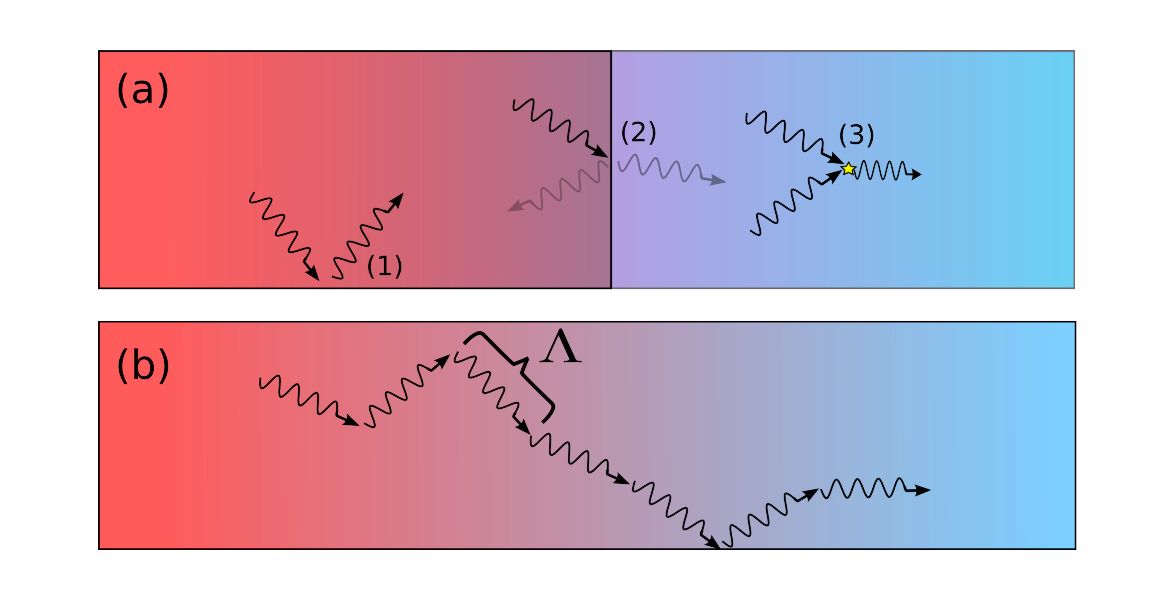
\includegraphics[width=.99\columnwidth]{inkscape/scattering.pdf}
 \caption{(a) Schematic illustration of microscopic scattering mechanisms in phononic thermal conduction: (1) Boundary scattering, (2) interface scattering, (3) phonon-phonon scattering. (b) Schematic of phonon propagation in a material, with scattering events at averages distances of mean free path $\Lambda$. \textbf{SCHEMATIC TO BE FINISHED, PERHAPS DRAW IN 2D FOR CLARITY}}
\label{fig:intro_scattering}
\end{center}
\end{figure}

The characteristic distance between phonon scattering events is called the phonon mean free path. While phonon mean free paths depend strongly on the material, temperature, vibrational frequency, and the type of scattering (elastic versus inelastic), a typical value for bulk silicon is around $\sim 300$ nm at room temperature \cite{ju99}. At length scales smaller than the mean free path, scattering events are too infrequent to drive phonon gas to local thermal equilibrium. Consequently, the classical Fourier's law of conduction \cite{fourier} based on the concept of a well-defined local temperature breaks down. 

Because of the relatively long intrinsic phonon mean free paths and the high surface-to-volume ratio of nanostructures, material interfaces and surfaces often have a dominant contribution to thermal resistance. Microscopically, phonon scattering at the interface between dissimilar materials arises both from atomic disorder at the interface and from the mismatch in the acoustic properties of the materials \cite{khalatnikov52}. Interfacial thermal resistance can present a bottleneck for the extraction of generated heat in electronic devices, thereby limiting their performance \cite{pop10}. Many methods have been suggested to reduce the thermal resistance between materials, including chemical functionalization \cite{hopkins11,kaur14,han15b}, external pressure \cite{shen11,chalopin12}, and heat-mediating thin films \cite{english12}. 

In a similar way, boundary scattering from material surfaces can strongly reduce the thermal conductivity in nanowires and thin films. Because efficient conversion of waste heat to electricity requires materials with a low thermal conductivity (and high electrical conductivity) \cite{chen}, low-dimensional materials such as silicon nanowires have been suggested to provide attractive platforms for thermoelectric modules \cite{hochbaum08,boukai08}. To reduce the thermal conductivity of nanowires even further, additional structuring such as alloying \cite{garg11}, partial amorphization \cite{donadio09}, and coating \cite{hu11} have been suggested.

% Because such reduction is expected to increase the thermoelectric figure of merit \cite{chen}, low-dimensional materials such as silicon nanowires have been suggested to be attractive materials for thermoelectric conversion \cite{hochbaum08,boukai08}. To reduce the thermal conductivity of nanowires even further, additional structuring such as alloying \cite{garg11}, partial amorphization \cite{donadio09}, and coating \cite{hu11} have been suggested.  % , but with care so that electrical conduction is not too strongly hindered. % depicted in Fig. \ref{fig:intro_hochbaum}. %\citepub{spectral}\citepub{twinning} % The diffusive scattering from the atomically rough surfaces reduces the thermal conductivity of silicon nanowires by two orders of magnitude compared to the bulk value  \cite{hochbaum08}.

Efficient extraction of heat from electronic devices requires not only small interfacial resistances but also bulk materials with high thermal conductivities \cite{pop10}. Nanomaterials with long phonon mean free paths are good candidates for such thermal management. For example, the rigid sp$^2$ bonding of carbon atoms in carbon nanotubes \cite{iijima91} gives rise to a thermal conductivity in the range of 500-5000 W/mK \cite{marconnet13}. Because of the very long mean free paths, however, the measured thermal conductivities depend on the tube length \cite{chang08}, with size-dependent variations observed even in millimeter-long nanotubes \cite{chang_personal}. It is even possible that the thermal conductivity of pristine carbon nanotubes diverges as a function of tube length, a signature of anomalous thermal conduction observed in computer simulations for one-dimensional atomic chains \cite{lepri03,mai07,dhar08}. Indications of anomalous thermal conduction were recently observed experimentally \cite{xu14} for graphene, the two-dimensional allotrope of carbon.

% Classical heat equation \eqref{eq:fourier} follows from the conservation of energy accompanied by Fourier's law of diffusion \cite{fourier}
% \begin{equation}
%  \mathbf{q} = -\kappa \nabla T(\mathbf{r},t),
% \end{equation}
% stating that local heat flux $\bb{q}$ is proportional to the negative temperature gradient. Fourier's law is built on the assumption that the local temperature $T(\bf{r},t)$ can be sensibly defined. Because temperature is a statistical quantity properly defined only for large systems \cite{}, the law must break down at small enough length scales. 

% The microscopic theory of thermal conduction was developed by Rudolf Peierls in 1929 \cite{peierls29}. Understanding that collective lattice vibrations (phonons) carry heat in crystalline solids, he proposed that thermal resistivity arises from the scattering of phonons from lattice imperfections and other phonons. These scattering mechanisms existing in any non-ideal material at non-zero temperature give rise to a finite phonon mean free path, characterizing the average distance between scattering events. At length scales much larger than the mean free path, the heat carriers are expected to essentially perform a random walk with constant drift along the temperature gradient and heat transfer is well described by Fourier's local theory. At length scales smaller than the mean free path, on the other hand, phonons can travel without scattering and Fourier's theory must be invalid. Phonon mean free paths depend strongly on the material, vibrational frequency and temperature \cite{}, but a typical value for bulk silicon is around $\sim 300$ nm at room temperature \cite{ju99}. 

% Thermal conduction in macroscopic systems is traditionally described using Fourier's law \cite{fourier}, stating that the heat flux at any given point is proportional to the temperature gradient at the same point. The theory leads, however, to the unphysical phenomenon that a local temperature perturbation can propagate infinitely fast \cite{chen}, in direct contradiction to the finiteness of the speed of sound and also special relativity. This indicates that Fourier's theory must ultimately break down in nanoscale.

 %Some experiments have claimed to have observed such anomalous thermal conduction in silicon nanowires \cite{yang10}, but the evidence remains inconclusive. % In two-dimensional materials such as graphene, similar divergence is expected, and recent experiments and simulations for graphene have suggested this to be the case \cite{xu14}. %\citepub{cnt}

% \begin{figure}
% \begin{center}
%  %\includegraphics[width=8.6cm]{pics/schwab00_fig3.ps}
%  \includegraphics[width=8.6cm]{pics/schwab_fig3.pdf}
%  \caption{Thermal conductance measured as a function of temperature by Schwab \textit{et al.} \cite{schwab00}. In their experimental setup, heat was transferred through four nanowires with four acoustic modes in each carrying the heat. The measured conductance at low temperature is therefore $G=16g_0$, where $g_0$ is the conductance quantum. Reprinted with permission from Ref. \cite{schwab00}.}
% \label{fig:intro_schwab}
% \end{center}
% \end{figure}

% In systems smaller than the phonon mean free path, the scattering-free propagation of phonons is called ballistic transport, contrasting with the diffusive transport of Fourier-like systems. The most striking example of ballistic transport is the thermal conductance quantization, predicted theoretically by Rego and Kirczenow in 1998 \cite{rego98} and observed experimentally in 2000 by Schwab \textit{et al.} \cite{schwab00} (see Fig. \ref{fig:intro_schwab}), thereby indirectly confirming also the existence of ballistic transport. 

% The thermal conductance quantum, which is analogous to the quantum of electrical conductance, is independent of any material properties and only depends on temperature and Planck's constant.  Their calculations showed that at sufficiently low temperatures, where phonon scattering is minimal and only the lowest-frequency phonon modes can be excited, thermal conductance through a narrow constriction is an integer multiple of the thermal conductance quantum. 

% As noted above, heat transfer is expected to be well described by Fourier's law in sufficiently large system. This ballistic-diffusive transition has been observed in bulk-like three-dimensional systems using computer simulations \cite{saito10}. In low-dimensional systems, on the other hand, computer simulations \cite{lepri97,lepri03,mai07,dhar08} and heat transfer experiments \cite{yang10,xu14} have indicated that the Fourier limit may never be reached. In one-dimensional oscillator chains, for example, it is now widely accepted \cite{dhar08} that the thermal conductivity diverges as a function of system length following a power-law \cite{mai07}, called anomalous thermal conduction \cite{dhar08}. It is, however, still debated \cite{marconnet13} if any physical system such as a nanowire can be treated as a one-dimensional object and could therefore exhibit the divergence.

% Nanostructure
\change{For applications in thermionic \cite{zeng06}\cite{westover08} and thermophotonic \cite{oksanen08} cooling, good thermal insulation between materials separated by nanoscale gap is required. Nanoscale point contacts bridging the vacuum gap and providing structural support are a good alternative due to their small thermal conductance \cite{bartsch12}. In such small structures, the wave nature of phonons cannot be neglected and interference effects appear. While there are earlier works investigating the thermal conductance of point contacts} \cite{bartsch12,jeong12}, \change{interference effects have not been addressed. Recognizing interference effects in point contacts could enable thermal conductivity engineering in a similar way as, e.g., in silicon thin films decorated with local resonators \cite{davis14}.}

% In point contacts with diameter around 10 nm \cite{bartsch12}, both phonon mean free path and dominant wavelength can largely exceed the contact size. 

% designing acoustic reflectors with novel applications in phonon lasing \cite{maryam13}, enhancing the optical-mechanical coupling \cite{fainstein13}, and phonon nanocapacitors \cite{han15}. 

% \textbf{ADD SHORT DISCUSSION OF POINT CONTACTS AS THERMAL BARIERS, PERHAPS BEGIN THE PARAGRAPH FROM POINT CONTACTS?}

% In addition to the mean free path, there is another important length scale governing heat transfer in microscopic scale: the phonon wavelength. In bulk silicon, the characteristic wavelength of thermally excited phonons is around 10 nm at room temperature \cite{ju99}. 

% Wavelength-related effects are also exploited in thermal engineering: as an example, Kim \textit{et al.} were able to reduce the thermal conductivity of InGaAs alloy, which naturally scatters short-wavelength phonons due to point defects, by introducing nanoparticles acting as scatterers for mid-to-long-wavelength phonons \cite{kim06}. %\citepub{fpu}\citepub{fpu2}\citepub{gf} % Other examples of interference

% \begin{figure}
% \begin{center}
%  %\includegraphics[width=8.6cm]{pics/schwab00_fig3.ps}
%  \includegraphics[width=.80\columnwidth]{pics/hochbaum_fig1.pdf}
%  \caption{(a) Scanning electron microscope image of a silicon nanowire array. (b) Transmission electron microscope image of a single nanowire, showing the prominent edge roughness responsible for strong phonon scattering. The low thermal conductivity gives rise to a high thermoelectric figure of merit. The electron diffraction pattern in the inset shows that the wire single crystalline along its length. Reprinted with permission from Ref. \cite{hochbaum08}.}
% \label{fig:intro_hochbaum}
% \end{center}
% \end{figure}



% Relation to the thesis
% Concepts such as phonon interference, ballistic transport, mean free paths, and interface scattering appear throughout this thesis. In Publications \cp{fpu}, \cp{fpu2}, and \cp{gf}, we explore the interference effects exhibited in thermal conduction through nanoscale constrictions and reveal intricate interference patterns in local nonequilibrium temperature profiles. We also show how such patterns vanish at higher temperatures due to increased scattering. In Publication \cp{spectral}, we present detailed maps of the contributions of different vibrational frequencies to thermal conduction across a mass-mismatched interface, improving thereby the understanding of heat transfer mechanisms at interfaces and presenting guidelines for future thermal engineering of high-conductance interfaces. Publication \cp{cnt} presents a non-equilibrium method for determining the mean free paths of phonons in carbon nanotubes, supplying a theoretical description of the ballistic-diffusive crossover in one-dimensional systems. In Publication \cp{twinning}, we perform ''thermal engineering'' and demonstrate the existence of minimun thermal conductivity at a certain twinning period length in a silicon nanowire. The minimun arises from the maximal blocking of bulk-like scattering-free propagation of phonons through the nanowire by the periodically repeating twinning boundaries.


%As noted by Kapitza already in 1930s \cite{}, carrier scattering at interfaces between materials also gives rise to thermal resistance. Even in the absence of defects, 

% Point contacts \cite{bartsch12}

% Contact resistance is a bottleneck
% Material properties increasingly dominated by interfaces

% Interfaces

% Superlattices, phonon mirrors

% While there is convincing evidence from numerical simulations that the Fourier limit is always achieved in three-dimensional systems \cite{saito10,wang10}, this seems not to be the case in one- or two-dimensional systems. Numerical simulations \cite{lepri97,mai07} and hydrodynamical theory \cite{} suggest that the thermal conductivity in one-dimensional systems diverges in a power-law fashion as a function of system length, but clear experimental demonstration of the divergence has not been achieved so far. In two-dimensional systems, thermal conductivity is expected to diverge logarithmically \cite{}. Recent experiments claim to have observed the divergence in graphene \cite{xu14}.

%\subsection{Thermal boundary resistance}

%\subsection{Thermal engineering}

\subsection{Electromagnetic energy transfer in the near-field}
\label{sec:intro_em}

Unlike lattice vibrations, electromagnetic fields can propagate and transfer heat even in vacuum. This phenomenon is best observed on a sunny day when the electromagnetic radiation emitted from the Sun heats the skin. \change{Like Sun, any object at non-zero temperature emits thermal radiation with a wide spectrum of wavelengths. According to Wien's law \cite{}, the spectrum of emitted thermal radiation peaks at a wavelength $\lambda_{\textrm{max}}$ that is inversely proportional to the object's temperature $T$. While $\lambda_{\textrm{max}}$ is around 500 nm for the Sun ($T\approx 5800$ K), objects at room temperature emit thermal radiation in the micrometer range.} % Like a miniature Sun, all matter radiates heat due to thermal excitation and fluctuations in electrons and nuclei in any matter undergo accelerating motion due to thermal fluctuations, all matter radiates heat like a miniature Sun. 

% While lattice vibrations cannot transfer heat without a medium, electromagnetic fields can propagate even in vacuum. Because all materials emit electromagnetic radiation due to the microscopic fluctuations of electrons and nuclei, 

\begin{figure}
\begin{center}
 %\includegraphics[width=8.6cm]{pics/schwab00_fig3.ps}
 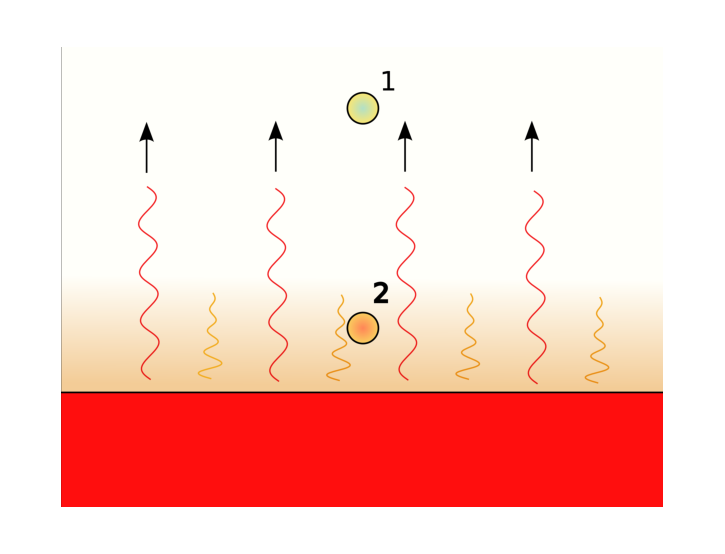
\includegraphics[width=.80\columnwidth]{inkscape/thermal_radiation.pdf}
 \caption{Due to microscopic thermal fluctuations, an object at non-zero temperature emits thermal radiation in the form of propagating electromagnetic waves (red), which can carry energy to objects at large distances (blue). Close to the object, there are, however, also evanescent waves (orange) with zero propagation velocity. If another object is placed in the near-field (black), the contribution of evanescent waves to energy transfer between the bodies can dominate over the propagating wave contribution. \textbf{SCHEMATIC TO BE FINISHED}}
\label{fig:intro_em}
\end{center}
\end{figure}

% Thermal radiation emitted from an object typically contains a wide range of photon wavelengths, with the distribution governed by the Planck distribution \cite{planck00a} and the wavelength-dependent emissivity of the object \cite{}. For objects at room temperature, the wavelength of emitted propagating waves are typically in the micrometer-range \cite{}.
\change{For two objects at different temperatures in vacuum and separated by a distance much larger than $\lambda_{max}$, the rate of energy flow from the hotter object to the colder one can be calculated from the energy carried by propagating electromagnetic waves \cite{}. Due to the lossless propagation of waves, this contribution is essentially independent of distance when the appropriate geometrical factors are accounted for \cite{}. At distances smaller than $\lambda_{\textrm{max}}$, however, evanescent waves localized close to each object \cite{novotny} can also contribute to energy transfer as depicted in Fig. \ref{fig:intro_em}. While these evanescent waves are ''invisible'' in the far-field and cannot carry energy far from the object due to their zero group velocity, their contribution to energy transfer can overwhelm the contribution of propagating waves at subwavelength distances (near-field).} %Therefore, energy transfer between materials is expected to be enhanced at submicrometer separation compared to the far-field value. 

The near-field enhancement of energy transfer was first observed by Hargreaves \cite{hargreaves69}, who measured the thermal conductance between two chromium layers separated by a micrometer-scale gap. The theoretical calculation for the exact enhancement rate was carried out by Polder and van Hove \cite{polder71}, and consequently near-field enhancement effects were predicted in numerous geometries \cite{loomis94,pendry99,carminati99,shchegrov00,mulet01,volokitin01}. In the last decade, advances in experimental techniques have allowed for very precise measurements of near-field enhancement rates \cite{kittel05,hu08,shen09,ottens11}, confirming theoretical predictions. 

In addition to existing applications in, e.g., thermal microscopy \cite{majumdar99,muller-hirsch99,kittel05,kittel08} and infrared thermophotovoltaics \cite{dimatteo01,narayanaswamy03,laroche06}, near-field effects are expected to be exploitable also in nanoscale thermal management, with possible applications in heat-assisted chemistry \cite{cao07,adleman09} and hyperthermic treatment of cancer \cite{vanderzee02}. The strong near-field interaction allows, for example, for the quick dissipation of heat from a heated nanoparticle to its near surroundings \cite{mulet01,domingues05}. Because of the short-ranged nature of the near-field, the enhanced coupling is, however, limited to very small distances. It has been suggested that thermal coupling between bodies could be further enhanced by the introduction of additional nanoparticles  \cite{benabdallah11,messina13} or heat-mediating thin films \cite{zheng11,messina12}. 

% and they are also expected to give rise to engineering applications in, e.g., infrared thermophotovoltaics \cite{dimatteo01,narayanaswamy03,laroche06} and designing narrow-band infrared antennas \cite{greffet02}. 



% The near-field enhancement of energy transfer was first observed experimentally by Hargreaves in 1969 \cite{hargreaves69} and described theoretically by Polder and van Hove in 1971 \cite{polder71} using Rytov's theory \cite{rytov} of fluctuational electrodynamics. 

% Far from a thermally radiating object, only the propagating electromagnetic waves emitted by the object carry energy. At wavelengths smaller than the dominant wavelength in thermal radiation, which is typically in the micrometer range at room temperature \cite{},   % the amount of energy radiated by a solid is given by the radiative heat transfer theory \cite{}, based on Max Planck's work \cite{planck00a} on blackbody radiation. 

% Accelerating charges are known to emit electromagnetic radiation \cite{jackson}. Because the electrons and nuclei in any solid material undergo thermal (and quantum) fluctuations, all materials therefore emit electromagnetic radiation carrying heat. Accurate theoretical description of the emitted electromagnetic spectrum was achieved by Max Planck in 1900 \cite{planck00a}. His blackbody radiation law played a key role in the development of quantum theory and describes, for example, the spectrum of cosmic microwave background radiation at the accuracy of XXX.


% \begin{figure}
% \begin{center}
%  %\includegraphics[width=8.6cm]{pics/schwab00_fig3.ps}
%  \includegraphics[width=8.6cm]{pics/kittel_fig1.pdf}
%  \caption{(a) Electric field lines close to a polar surface with positive (green) and negative (red) charges. (b) The strength of electric field as a function of distance from the surface, showing the localization close to the surface. Reprinted with permission from Ref. \cite{kittel09}.}
% \label{fig:intro_kittel}
% \end{center}
% \end{figure}
% In 1900, Max Planck \cite{planck00a} studied the radiation emitted by a perfectly absorbing medium and gave birth not only to quantum theory but also to Planck's blackbody radiation law, which has since been observed to describe, for example, the spectrum of cosmic microwave background radiation at the accuracy of XXX.
% 

% Planck's law inherently suggests that the total power of the emitted radiation is independent of the distance from the object. This follows from the assumption that only propagating electromagnetic waves contribute to the energy density. Close to the material surface, solution of Maxwell's equations gives, however, also rise to evanescent electromagnetic fields localized at a distance of a few wavelengths from the object \cite{polder71} as depicted in Fig. \ref{fig:intro_kittel}. One can then envisage placing another object sufficiently close to the radiating body so that the evanescent fields can induce motion of charges in the added object, leading to energy transfer by the evanescent fields. Planck's law therefore breaks down at very small distances. 



% \begin{figure}
% \begin{center}
%  %\includegraphics[width=8.6cm]{pics/schwab00_fig3.ps}
%  \includegraphics[width=8.6cm]{pics/shchegrov00_fig1.pdf}
%  \caption{The spectral energy density of electromagnetic field (arbitrary units) close to a SiC surface at distances of (a) $1$ mm, (b) $2$ $\mu$m, and (c) $100$ nm. At the distance of 100 nm, the spectral energy density is dominated by the surface phonon polariton at frequency $\omega=178.7$ Trad/s, resulting in essentially monochromatic energy emission. Inset show the spectral energy densities plotted in semilogarithmic scale. Reprinted with permission from Ref. \cite{shchegrov00}.}
% \label{fig:intro_shchegrov}
% \end{center}
% \end{figure} 

% Near-field effects are particularly strong for materials supporting evanescent surface waves decaying at both sides of the surface \cite{shchegrov00}. The surface waves arise from the coupling between the electromagnetic field and either the free electrons (surface plasmon polaritons) or transverse optical phonons (surface phonon polaritons). While surface plasmon polaritons can only be thermally excited in metals at temperatures much higher than room temperature, surface phonon polaritons can contribute to thermal transfer in polar semiconductors even at room temperature. To demonstrate the large contribution of surface waves, Fig. \ref{fig:intro_shchegrov} shows the theoretically calculated \cite{shchegrov00} spectral energy density of the electromagnetic field at various distances from a SiC surface.

% Similarly, near-field effects strongly increase the spectral density of the electromagnetic field in the vicinity of nanoparticles made of a polar material. Consequently, heat transfer between two nanoparticles in vacuum is found to strongly increase at small distances \cite{domingues05}. In practice, however, the required nanoparticle distances for efficient heat transfer may be too small, so for practical applications it would be necessary to engineer the thermal conductance to be higher. From the theory of dipole emission, it is well known that the optical-mechanical coupling can be enhanced by orders of magnitude in an inhomogeneous environment such as in a mirror cavity \cite{novotny}. This raises the question, if the interparticle heat transfer rate between particles could be enhanced by cavity. This question was investigated and answered in positive in \citepub{dipole}.


\subsection{Electronic effects in heat transfer}
\label{sec:intro_electrons}

\change{The density of transistors in state-of-the-art microchips has increased exponentially for more than four decades, powering the digital revolution. The increase in transistor density and operating frequency have lead to an exponential increase in the dissipated power density as well, increasing the power consumption of CPUs and requiring drastic cooling  solutions in datacenters \cite{pop10}. While the increase in dissipated power has slowed down by the introduction of multi-core CPUs, proper management of the unwanted heat at both chip and individual transistor level is still an essential ingredient of modern electronics design \cite{pop06_ieee}.}

%  exceeding 100 W/cm$^2$ around 2005 \cite{pop10} and . For comparison, the power dissipated by a hot plate is around 10 W/cm$^2$. 
% What is electronic self-heating?
Microscopically, electronic heating arises from the interactions between high-energy electrons and phonons. In silicon-on-insulator transistors, for example, the electric field is known to be particularly strong close to the drain \cite{pop06_ieee}. As electrons accelerated by the strong electric field lose their energy by colliding with lattice vibrations, the excess energy is absorbed by the lattice. The resulting increase in lattice temperature gives rise to nanoscale hot spots with low electron mobilities \cite{pop06_ieee}, interfering with the device performance. % While electronic self-heating % silicon-on-insulator (SOI) transistors.

\change{Electron-phonon interactions play an important role also in thermal conduction across metal-dielectric interfaces. Electrons can contribute to interfacial energy transfer either directly by interacting with the phonons in the dielectric or indirectly by exchanging energy with phonons in the metal, which can then carry vibrational energy across the interface} \cite{huberman94,sergeev98,mahan09}. \change{Computational modeling of such electron-phonon energy exchange in complex systems has been carried out mainly by Monte Carlo simulations and classical two-temperature models (see, e.g., Refs. \cite{sadi06}\cite{guo12} and references therein), which both neglect the wave nature of electrons and are therefore of limited applicability in nanometric structures.}

% While electron-phonon interaction reduces the mobility of charge carriers and is therefore detrimental in applications, electron-photon interaction drives all optoelectronic applications such as light-emitting diodes, lasers and solar cells. \textbf{WRITE SOMETHING ABOUT THE NEEDS OF MICROSCOPIC ELECTRO-OPTICAL MODELS...}

% Self-heating is not, however, only a nuisance, as the local temperature profiles modified by self-heating give quantitative information of the microscopic electron transport in the device under study. Local temperature profiles can be probed, for example, by scanning Joule expansion microscopy \cite{varesi98}, Raman scattering spectroscopy \cite{calizo07} or by measuring the local infrared emission \cite{bae10}. These methods have been used to produce detailed temperature maps in biased low-dimensional nanomaterials such as carbon nanotubes \cite{estrada11,xie12} and graphene \cite{bae10,freitag09,chae10,freitag10}.

%Interaction of electrons with photons, on the other hand, drives all optoelectronic applications such as light-emitting diodes, lasers and solar cells. 
%\textbf{WRITE ABOUT THE NEEDS OF MICROSCOPIC ELECTRO-OPTICAL MODELS.}

% \textbf{HOW TO TIE THIS ALL TO THE THESIS?}

% Self-heating is not, however, only a nuisance, as the local temperature profiles affected by self-heating give quantitative information of the microscopic electron transport in the device under study. Local temperature profiles can be probed, for example, by scanning Joule expansion microscopy \cite{varesi98}, Raman scattering spectroscopy \cite{calizo07} or by measuring the local infrared emission \cite{bae10}. These methods have been used to produce detailed temperature maps in biased low-dimensional nanomaterials such as carbon nanotubes \cite{estrada11,xie12} and graphene \cite{bae10,freitag09,chae10,freitag10}.

% As an example of microscopic heating effects, consider electron transport in the silicon-on-insulator (SOI) transistor depicted in Fig. \ref{fig:soi}. The strong electric field close to the drain accelerates electrons, giving rise to so-called hot electrons \cite{}. As these electrons collide with phonons and thereby give their energy to the lattice at distances of multiple inelastic electron mean free paths, lattice temperature increases and reduces electron mobility close to the drain, decreasing the device performance. 

% \begin{figure}
% \begin{center}
%  %\includegraphics[width=8.6cm]{pics/schwab00_fig3.ps}
%  \includegraphics[width=8.6cm]{pics/grosse_fig1.pdf}
%  \caption{(a) Optical image of a two-grain graphene flake (dark gray) between Pd electrodes (bright). The grain boundary (GB) is shown by the dashed line. (b) Measured surface expansion $\Delta h$ (color) overlaid on the device topography. The surface expansion is proportional to the local temperature rise, revealing Joule heating at the grain boundary. Reprinted with permission from Ref. \cite{grosse14}.}
% \label{fig:intro_grosse}
% \end{center}
% \end{figure} 

 % As an example, Fig. \ref{fig:intro_grosse} shows the local surface expansion profile, proportional to the local temperature, measured using scanning Joule expansion microscopy at a graphene grain boundary \cite{grosse14}.

% Theoretical description of electron transport in nanoscale is similar to phonon transport: interference effects and ballistic transport appear at length scales dictated by the carrier wavelength and mean free path, respectively. \cite{} It is also often the case that the electron mean free path is in the range of device's characteristic dimensions, implying that electron transport cannot be modeled as fully ballistic or diffusive \cite{}. In such cases, models accounting for both wave-like behaviour and partially ballistic transport are required. 

% \begin{itemize}
%  \item LITERATURE OF ELECTRON INTERFERENCE EFFECTS IN SUPERLATTICES? (no Aharonov-Bohm or weak localization...)
% \end{itemize}


% In materials with electrostatically tunable Fermi levels such as graphene, electron wavelength can exceed $xXX$ nm \cite{}, requiring full wave picture of carrier transport in nanoscale graphene devices. 

% \subsection{Interplay of carriers in nanoscale}
% \label{sec:intro_coupling}
% \begin{itemize}
%  \item Electron-phonon effects on dielectric-metal interface and in laser heating, two-temperature models, necessity of more microscopic models
%  \item Photon-phonon effects at vacuum gaps, Green's function models, correct description of radiation-conduction crossover, acoustic phonon tunneling, two-temperature models?
%  \item Electron-photon models (situation where including an electromagnetic field in tight-binding Hamiltonian is necessary?)
%  \item Envisage the inclusion of all carriers, three-temperature models?
% \end{itemize}



\section{Studied structures}

\begin{figure}
\begin{center}
 %\includegraphics[width=8.6cm]{pics/schwab00_fig3.ps}
 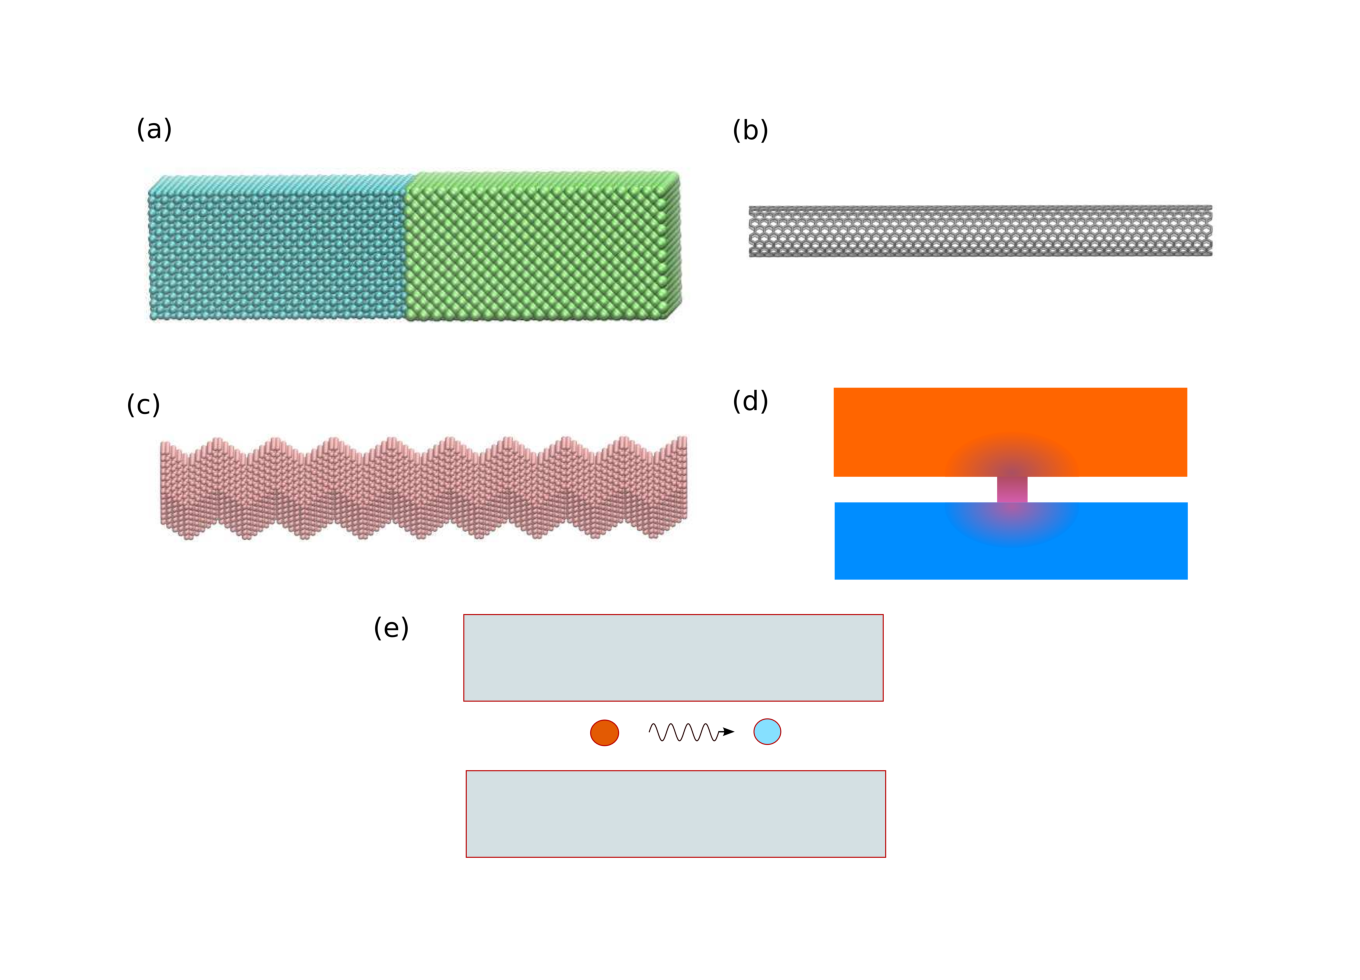
\includegraphics[width=.99\columnwidth]{inkscape/systems.pdf}
 \caption{Schematic illustration of the structures investigated in this work. (a) Interface between two crystals with different masses, (b) carbon nanotube, (c) silicon nanowire with periodic twinning, (d) point contact connecting bulk materials, and (e) cavity-enhancement of electromagnetic energy transfer between nanoparticles. \textbf{ATOMISTIC ILLUSTRATIONS TO BE FINISHED}}
\label{fig:intro_structures}
\end{center}
\end{figure}

The structures investigated in the publications of this thesis are depicted in Fig. \ref{fig:intro_structures}. The broad topics concerning each depicted structure were, corresponding to figure labeling, (a) interfacial thermal resistance, (b) phonon mean free paths in nanotubes, (c) thermal conductivity engineering in nanowires, (d) phonon interference effects in point contacts, and (e) electromagnetic energy transfer in cavity. % Each of the structures and the main results are briefly reviewed below. 
% Publications \cp{spectral}--\cp{gf} focus on phononic thermal conduction. 

The interface structure of Fig. \ref{fig:intro_structures}(a) is used as the simulation geometry to study the role of phonon-phonon scattering in interfacial thermal conduction between two bulk crystals with different masses. The results of \citepub{spectral} show that phonon-phonon scattering can reduce the resistance via two mechanisms, namely (1) dissipation of evanescent vibrational modes localized close to the interface, and (2) energy-doubling and energy-halving three-phonon scattering processes carrying energy across the interface.  % Energy transfer mechanisms at the interface are identified by determining the spectral decomposition of energy current at the interface using the spectral analysis methods developed in \citepub{spectral}. T

The carbon nanotube structure schematically depicted in Fig. \ref{fig:intro_structures}(b) is used in the simulations of \citepub{cnt} to determine the phonon mean free paths in carbon nanotubes. The mean free paths were determined from non-equilibrium simulations by utilizing the spectral analysis methods developed in \citepub{spectral}. The mean free paths in carbon nanotubes were shown to exceed 0.01 mm at low frequencies, with possibly even longer mean free paths at lower frequencies. The results suggest that very long, millimeter-scale nanotubes can be even better thermal conductors than expected. % The results also indicated that the relaxation times determined from the decay of non-equilibrium heat current differ, in general, from the relaxation times determined from the mode decay in equilibrium.
 
Figure \ref{fig:intro_structures}(c) shows a silicon nanowire with periodic twinning stacking faults, which create a zigzag-like structure impeding phonon flow and thereby reducing thermal conductivity compared to the straight wire. The atomistic simulations of \citepub{twinning} show that periodic twinning can reduce the thermal conductivity of Si nanowires by 65 \% at room temperature, suggesting that twinning could boost the thermoelectric efficiency of silicon nanowires. Twinning can also be paired with other structural modifications to reduce the thermal conductivity even further.

Thermal conduction through a nanoscale point contact, illustrated in Fig. \ref{fig:intro_structures}(d), is the topic of Publications \cp{fpu}, \cp{fpu2}, and \cp{gf}. For a point contact in a square lattice, interference effects are shown to give rise to directional features in the local temperature profile. As expected, interference features are washed away at higher temperature because of the increasing phonon-phonon scattering. Local temperature profile is also modified when the quantum-mechanical occupation function of heat carriers is taken into account. 

Figure \ref{fig:intro_structures}(e) illustrates two polar nanoparticles located in a microcavity. The calculations of \citepub{dipole} show that the cavity (i) increases the thermal coupling between nanoparticles and (ii) gives rise to non-monotonic thermal coupling as a function of nanoparticle distance arising from the interference of the standing cavity waves. The results suggest that modifying the electromagnetic environment can flexibly and efficiently tune the thermal coupling between electromagnetically coupled bodies.


%\subsection{Interfaces}

%\subsection{Carbon nanotubes and twinning nanowires}

%\subsection{Point contacts}

% \subsection{Nanoparticles in a mirror cavity}

%In bulk silicon, electron mean free path at room temperature is around 5--10 nm \cite{}, necessitating the accounting for ballistic electron transport in modern transistor designs with characteristic dimensions around 10 nm \cite{}. 

% Differences between microscopic and macroscopic electron transport are similar to phonon transport: interference effects and ballistic transport appear at length scales dictated by the carrier wavelength and mean free path, respectively. Contrary to phonons, however, only electrons in a given energy range around the Fermi energy typically contribute to the transport. Therefore, transport properties such as mean free path can often be approximated as energy-independent. %The important length scales are set by the Fermi wavelength and electron mean free path.

% For example, Pop \textit{et al.} utilized the strong self-heating at high voltage bias to determine the thermal conductance of suspended carbon nanotubes \cite{pop06}. Detailed temperature maps of biased carbon nanotubes and graphene have been obtained by scanning Joule expansion microscopy \cite{xie12} (based on measuring local thermal stresses using atomic force microscopy \cite{majumdar}), measuring thermal infrared emission \cite{freitag10} and from Raman scattering microscopy \cite{freitag09,chae10}. Joule heating has also been used to monitor current transport at graphene-metal interfaces \cite{grosse11}

% \cite{freitag10} Thermal infrared emission
% Metal-dielectric interfaces

% Due to the small size of the transistor, the electronic heating in transistors cannot be described using Fourier's law \cite{}. 



%Because of the partially ballistic electron transport in such small structures, electrons cannot dissipate their energy to the lattice as efficiently as estimated by Fourier's law \eqref{eq:fourier}. Nanoscale phenomena 

%Similarly to phonon transport, electron transport in macroscale is also described by the Fourier's law of diffusion \eqref{}. 

% Transistors become smaller
% Large electric fields accelerate electrons -> hot electrons -> interaction with phonons -> hot spots (not necessarily at the acceleration point)
% Electric fields especially at the drain
% Local Fourier law breaks down
% Small, complex structures with many materials (high-k dielectrics etc.), low thermal conductivities

% wave-damped model: account for wave properties and damping, Joule heating, thermoelectric effects, similar to hydrodynamic model + wave effects
% Neglects: which phonons are populated, interaction mainly with optical modes, lumps interactions into a single relaxation time (determined from mobility?)


\iffalse
\section{Summary of experimental techniques}

\subsection{Thermal conductivity}

\begin{itemize}
 \item $3\omega$ technique
 \item Picosecond ultrasonic techniques (transient reflectance)
\end{itemize}

\subsection{Local temperature}

\subsection{Electromagnetic near-field transfer}

\subsection{Scanning thermal microscopy}

Measure the temperature of an AFM probe during the scan using either a thermocouple junction (measure voltage caused by temperature change) or microbolometer technique (measure change in resistance). In the latter, two leads are connected at the end of the probe by a Joule heating element which can be used either for temperature measurement by measuring its temperature change or for heating by driving current through it. In the constant power mode, the resistance of the heating element is measured by measuring the voltage in a Wheatstone bridge. If the voltage is fed back to the contact voltage, one can keep constant temperature at the resistor. 

Heat flow from the tip can be due to
\begin{itemize}
 \item Solid-solid conduction (this is what is wanted)
 \item Liquid-liquid conduction by the liquid meniscus between the tip and the sample, use UHV conditions
 \item Gas-gas conduction, use UHV conditions
 \item Near-field radiation between the tip and the sample
 \item Heat flow to cantilever
\end{itemize}

If the temperature of the tip, say, drops during the scan, this can be due to (a) lower local temperature, or (b) higher thermal conductivity at the sample spot. Also lower heat capacity is possible (?). 

Technique developed by Nonnenmacher (1992), Wickramasinghe (1992), Majumdar (1993), Pilkki (1994), etc.

Other methods to measure temperature are (see the review by Yue and Wang)
\begin{itemize}
 \item Optical methods based on the temperature-dependence of Raman or fluorescence signal of the measuring target (molecule, nanoparticle, etc.), which can also be used as the temperature sensor at the tip of an AFM, for example
 \item Near-field optical temperature measurement, with or without aperture
\end{itemize}

\subsection{Inelastic neutron scattering}
 \begin{itemize}
  \item Neutrons interact strongly only with the atomic nuclei (dipole scattering etc. typically weaker)
  \item Map the change in the neutron energy and momentum, one-phonon scattering processes sharply resolved among the multi-phonon process background
  \item Vary neutron energy, orientation of crystal and detection direction
  \item Gives phonon dispersion relations and broadenings, anharmonic effects mapped recently e.g. in doi:10.1038/nmat3035 and doi:10.1038/nnano.2013.95
 \end{itemize}
\fi
